\documentclass[12pt,a4paper]{article}
\usepackage[utf8]{inputenc}
\usepackage{amsmath, amssymb}
\usepackage{geometry}
\usepackage{tikz}
\geometry{margin=2cm}

\title{Fissão Nuclear: Física, Cálculos e Visualização}
\author{Samuel Keullen Sales}
\date{\today}

\begin{document}

\maketitle

\section*{1. Introdução}

A \textbf{fissão nuclear} ocorre quando um núcleo pesado (como \(\mathrm{U^{235}}\) ou \(\mathrm{Pu^{239}}\)) absorve um nêutron e se divide em dois núcleos menores (fragmentos de fissão), liberando energia, radiação gama e nêutrons livres.  
Esta reação é base para reatores nucleares e armas nucleares.

---

\section*{2. Reação de Fissão}

Exemplo da fissão do \(\mathrm{U^{235}}\):

\[
{}^{235}\mathrm{U} + n \rightarrow {}^{236}\mathrm{U}^* \rightarrow {}^{141}\mathrm{Ba} + {}^{92}\mathrm{Kr} + 3 n + \text{energia}
\]

\begin{itemize}
    \item Núcleo absorve nêutron → fica excitado (\({}^{236}\mathrm{U}^*\))
    \item Divide-se em dois fragmentos menores
    \item Libera \(2-3\) nêutrons livres
    \item Energia liberada na forma de radiação, energia cinética e nêutrons
\end{itemize}

\begin{center}
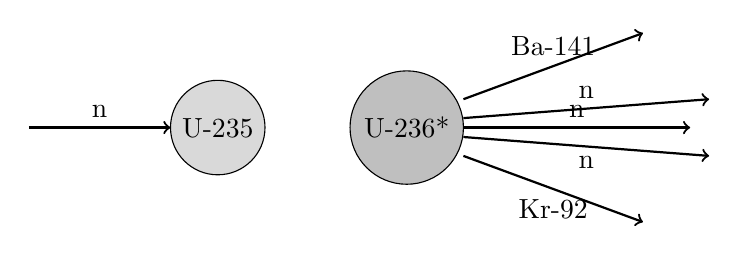
\begin{tikzpicture}[scale=1.2]
% Nucleo inicial
\draw[fill=gray!30] (0,0) circle (0.5);
\node at (0,0) {U-235};

% Neutron incidente
\draw[->, thick] (-2,0) -- (-0.5,0) node[midway, above]{n};

% Nucleo excitado
\draw[fill=gray!50] (2,0) circle (0.6);
\node at (2,0) {U-236*};

% Fissão
\draw[->, thick] (2.6,0.3) -- (4.5,1) node[midway, above]{Ba-141};
\draw[->, thick] (2.6,-0.3) -- (4.5,-1) node[midway, below]{Kr-92};
\draw[->, thick] (2.6,0.0) -- (5,0) node[midway, above]{n};
\draw[->, thick] (2.6,0.1) -- (5.2,0.3) node[midway, above]{n};
\draw[->, thick] (2.6,-0.1) -- (5.2,-0.3) node[midway, below]{n};
\end{tikzpicture}
\end{center}

---

\section*{3. Cálculo de Energia Liberada}

\subsection*{3.1 Diferença de Massa}

Dados:

\[
m_\text{U} = 235.0439\,\mathrm{u}, \quad
m_\text{Ba} = 140.9144\,\mathrm{u}, \quad
m_\text{Kr} = 91.9262\,\mathrm{u}, \quad
m_n = 1.0087\,\mathrm{u}
\]

\begin{align*}
\Delta m &= (m_\text{U} + m_n) - (m_\text{Ba} + m_\text{Kr} + 3 m_n) \\
&= 236.0526 - 236.8660 = -0.8134\,\mathrm{u}
\end{align*}

Energia liberada:

\[
E = |\Delta m| c^2 = 0.8134 \cdot 931.5 \approx 757.2 \,\mathrm{MeV}
\]

\subsection*{3.2 Energia Cinética dos Fragmentos}

Aproximadamente 85\% da energia vai para os fragmentos:

\[
E_\text{cin} = 0.85 \times 757.2 \approx 643.6 \,\mathrm{MeV}
\]

Distribuição proporcional à massa dos fragmentos.

\subsection*{3.3 Energia dos Nêutrons e Radiação Gama}

\begin{align*}
E_n &\approx 0.05 \times 757.2 \approx 37.9 \,\mathrm{MeV}, \quad \text{cada nêutron: } 12.6\,\mathrm{MeV} \\
E_\gamma &\approx 0.10 \times 757.2 \approx 75.7 \,\mathrm{MeV}
\end{align*}

---

\section*{4. Reação em Cadeia}

- Cada nêutron liberado pode induzir nova fissão.  
- Condição de reação crescente: massa crítica, geometria e material fissível.

Número médio de nêutrons por fissão: \(\nu \approx 2.5\)

\[
N(t) = N_0 \cdot (\nu)^n
\]

onde \(n\) é o número de gerações.

\begin{center}
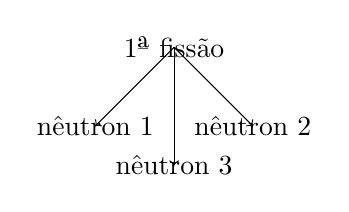
\begin{tikzpicture}[scale=1]
\node at (0,0) {1ª fissão};
\node at (-1,-1) {nêutron 1};
\node at (1,-1) {nêutron 2};
\node at (0,-1.5) {nêutron 3};

\draw[->] (0,0) -- (-1,-1);
\draw[->] (0,0) -- (1,-1);
\draw[->] (0,0) -- (0,-1.5);
\end{tikzpicture}
\end{center}

---

\section*{5. Tabela Resumo de Energia}

\begin{center}
\begin{tabular}{|c|c|}
\hline
Tipo de Energia & Valor (MeV) \\
\hline
Total & 757.2 \\
Cinética dos fragmentos & 643.6 \\
Nêutrons & 37.9 \\
Radiação Gama & 75.7 \\
\hline
\end{tabular}
\end{center}

---

\section*{6. Observações}

- Energia por núcleo fissionado: milhares de vezes maior que combustíveis químicos.  
- Fissão controlada: reatores nucleares.  
- Fissão descontrolada: bombas nucleares.  
- Visualização dos fragmentos e nêutrons ajuda a compreender a reação em cadeia e distribuição de energia.

\end{document}
